\begin{wrapfigure}{r}{0.2\linewidth}
	\centering
	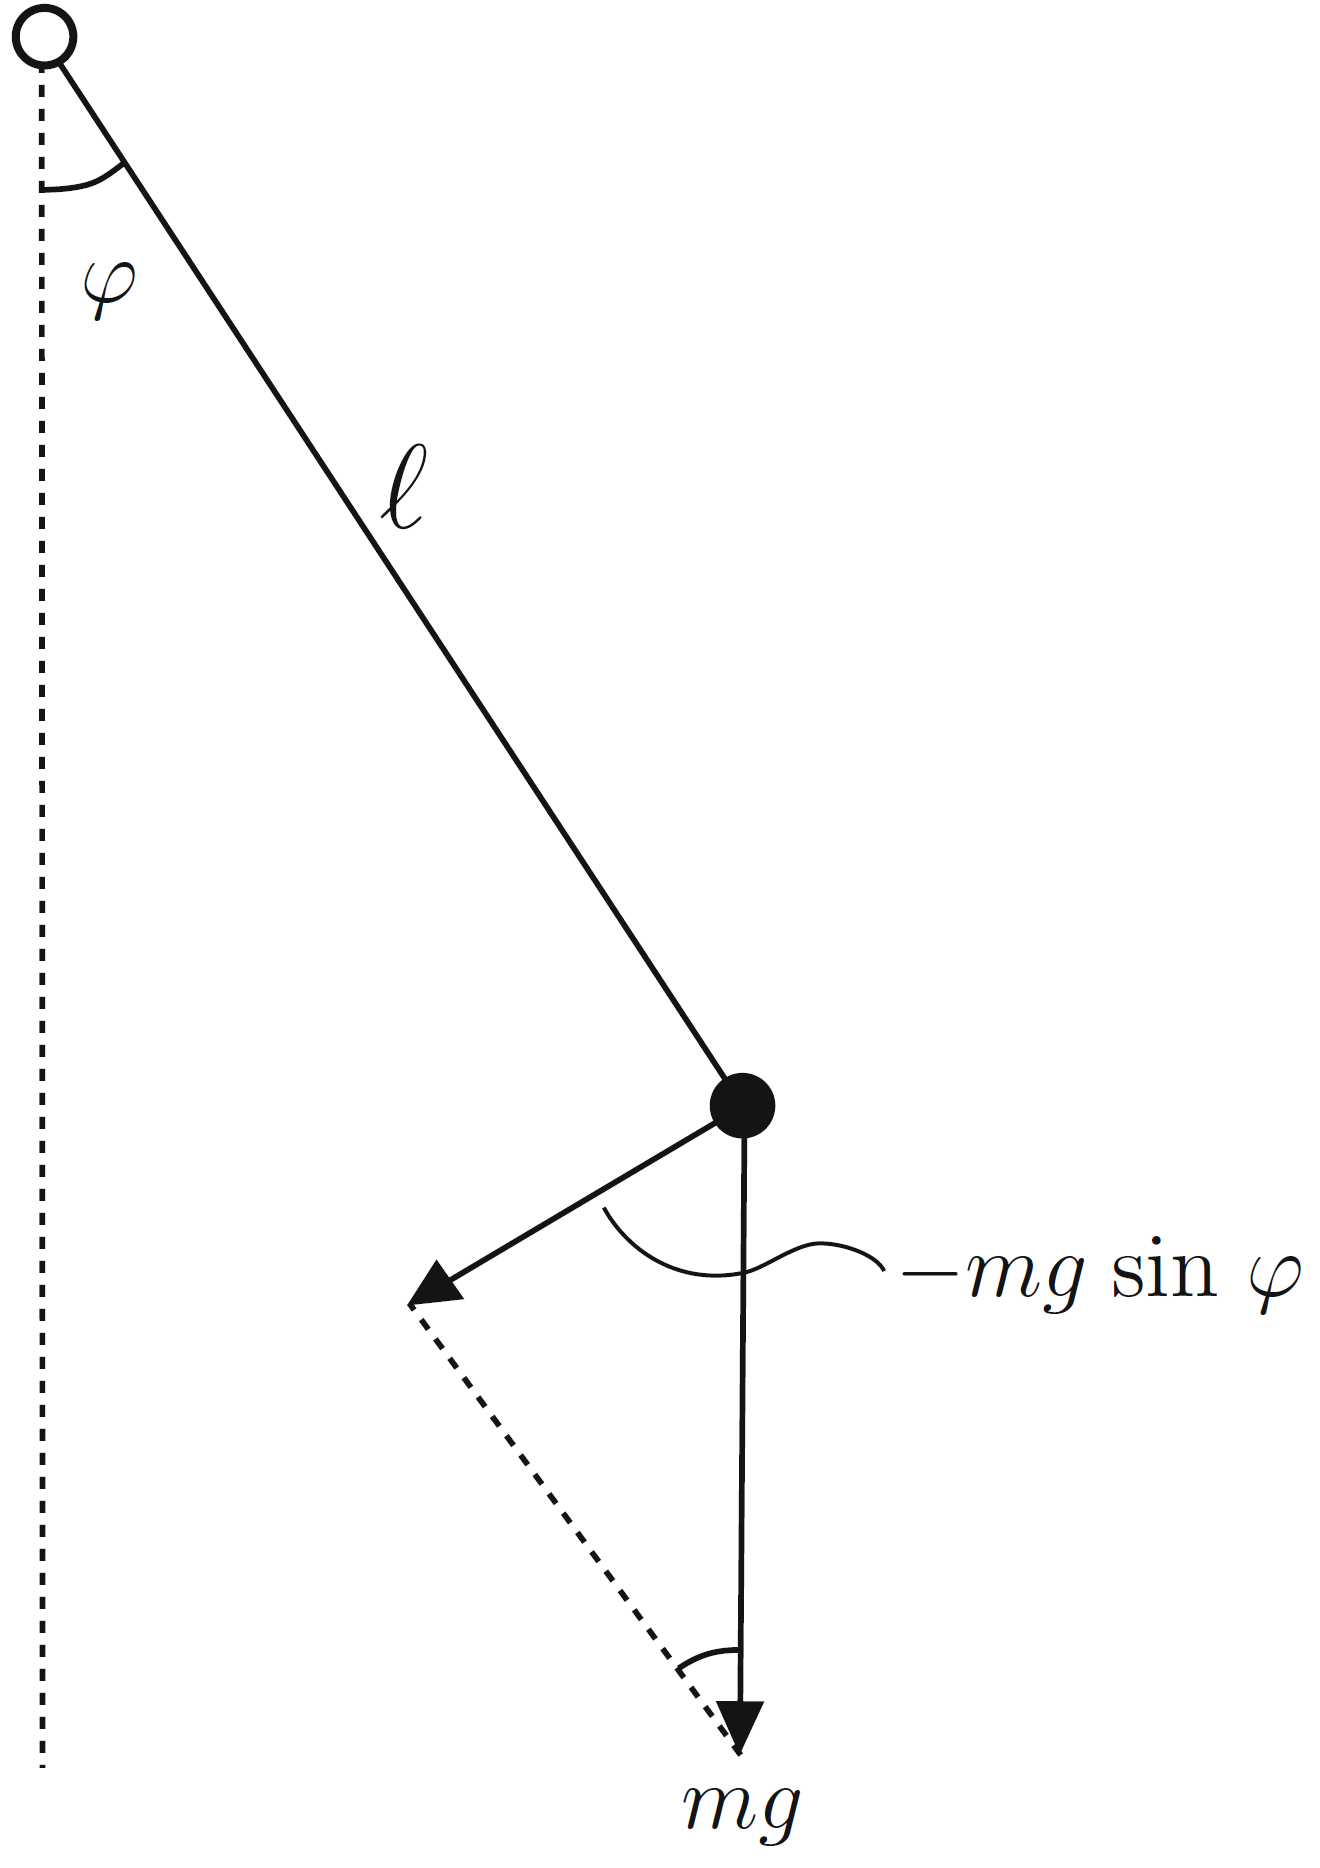
\includegraphics[width=\linewidth]{tfp.png}
	\caption{Sketch of the planar mathematical pendulum.}
	\label{fig:tfp}
\end{wrapfigure}
The planar mathematical pendulum consists of a rod, suspended at a fixed point in a vertical plane in which the pendulum can move.
All mass is thought of as being concentrated in a point mass at the end of the rod (see Figure (\ref{fig:tfp})), and the rod itself is massless.
Also the rod is assumed stiff.
The pendulum has mass $m$ and length $\ell$.
We moreover assume the suspension to be such that the pendulum not only can oscillate, but also can go `over the top'.
In the case without external forcing, we speak of the \emph{free} pendulum.
\subsubsection{The Free Undamped Pendulum}
In the case without damping and forcing the pendulum is only subject to gravity, with acceleration $g$.
The gravitational force is pointing vertically downward with strength $mg$ and has a component $-mg\sin\varphi$ along the circle described by the point mass (Figure \ref{fig:tfp}).
Here $\varphi$ is the angle between the rod and the downward vertical, often called \emph{deflection}.
The distance of the point mass from the \emph{rest position} ($\varphi=0$), measured along the circle of all its possible positions, then is $\ell\varphi$.
Applying Newton’s law in the $\varphi$-direction.
\begin{equation*}
	a=\frac{d^2(\ell\varphi)}{dt^2}=\ell\varphi^{\prime\prime}(t)\quad\rightarrow\quad
	m\ell\varphi^{\prime\prime}=-mg\sin\varphi\quad\rightarrow\quad
	\varphi^{\prime\prime}=-\frac{g}{l}\sin\varphi\quad\text{where $m,l>0$}
\end{equation*}
In Figure (\ref{fig:tfup}), the points ($2\pi k,0$), $k\in\mathbb{Z}$, correspond to the stationary motion (which rather amounts to rest and not to motion) where the pendulum hangs in its downward equilibrium.\\
The points ($2\pi \left(k+\frac{1}{2}\right),0$), $k\in\mathbb{Z}$, correspond to the stationary motion where the pendulum stands upside down.
\begin{figure}[h!]
	\centering
	\begin{subfigure}{0.4\linewidth}
		\centering
		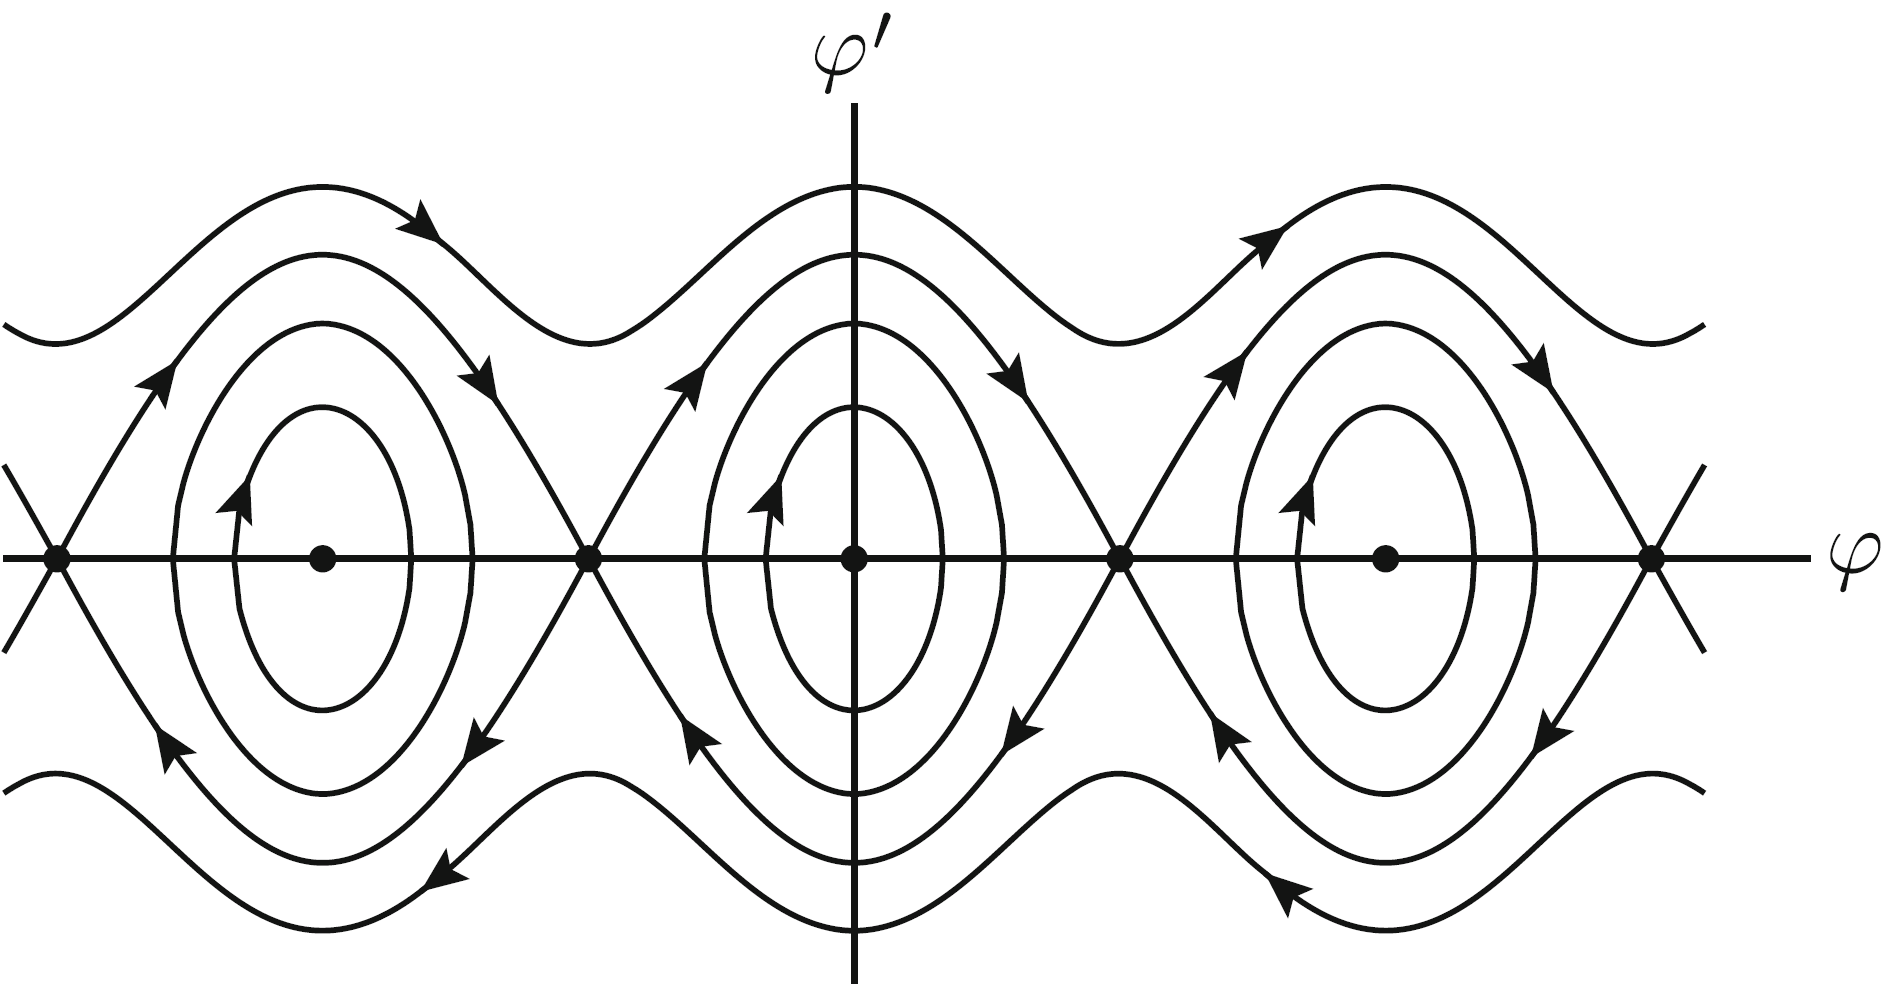
\includegraphics[width=\linewidth]{tfup.png}
		\caption{Curves in the Phase Plane}
		\label{fig:tfup}
	\end{subfigure}
	\vline
	\begin{subfigure}{0.36\linewidth}
		\centering
		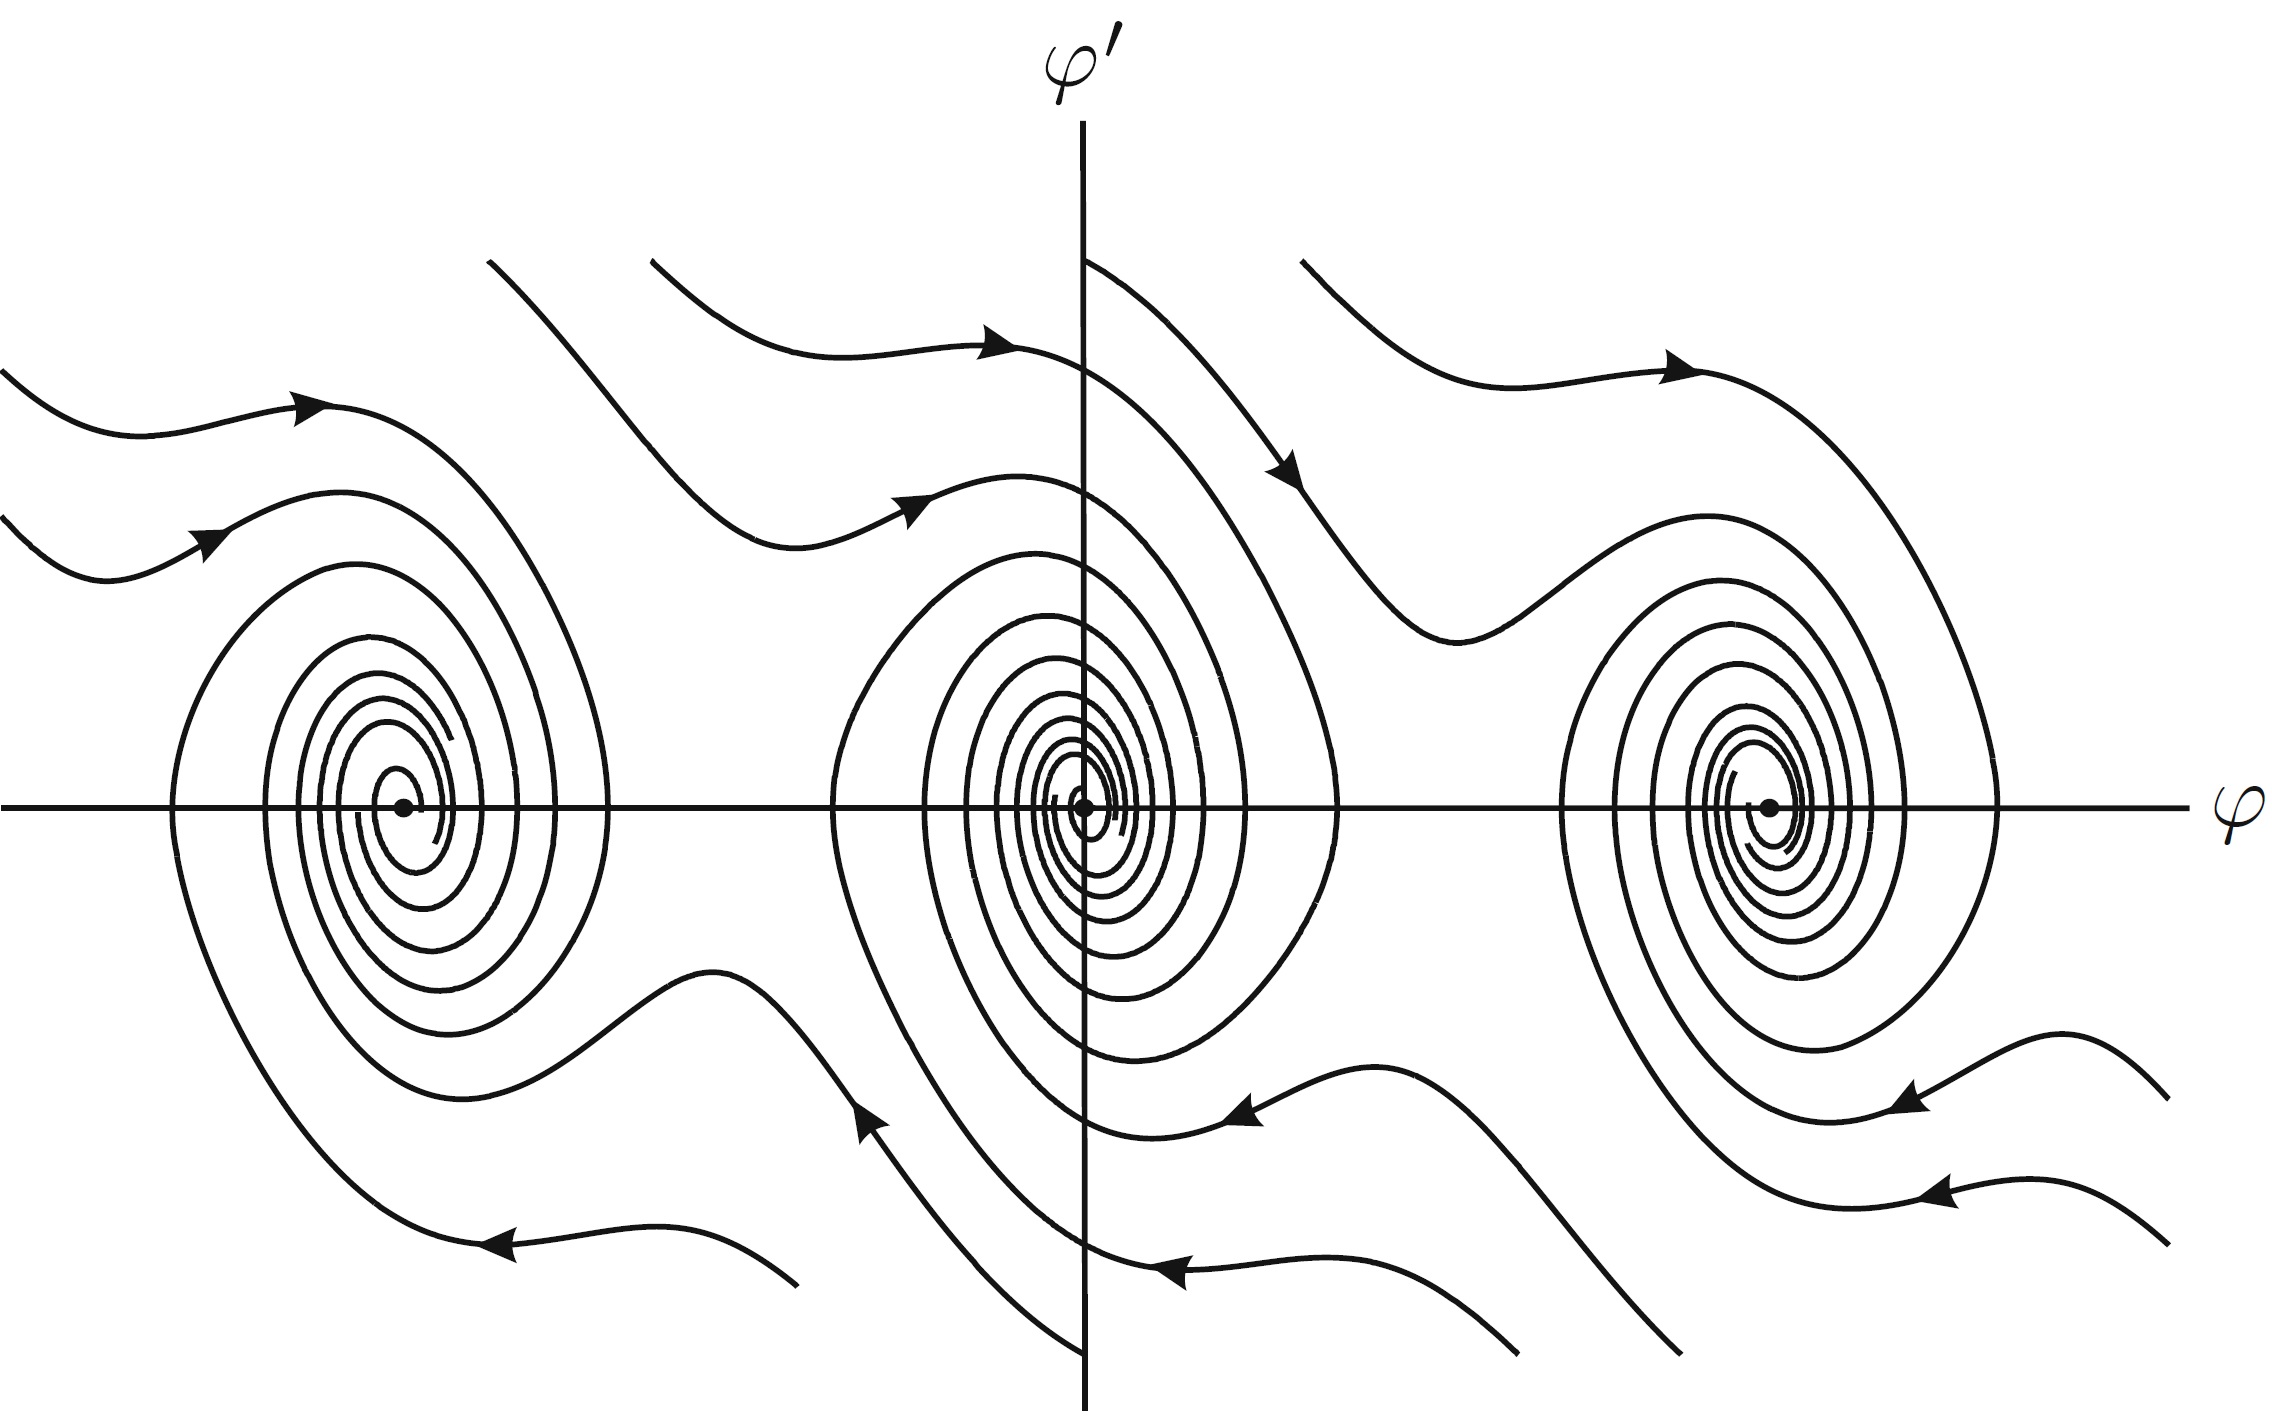
\includegraphics[width=\linewidth]{tfdp.png}
		\caption{Evolutions in the Phase Plane}
		\label{fig:tfdp}
	\end{subfigure}
	\caption{}
\end{figure}
\begin{remark}
	The natural state space of the pendulum really is a cylinder.
	In order to see that the latter curves are periodic, we have to make the identification $\varphi\sim\varphi+2\pi$ which turns the $(\varphi,\varphi^\prime)$-plane into a cylinder.
\end{remark}
\subsubsection{The Free Damped Pendulum}
In the case that the pendulum has damping, dissipation of energy takes place and a possible motion is bound to converge to rest.
For simplicity it is here assumed that the damping or friction force is proportional to the velocity and of opposite sign.\\
The equation of motion is given by
\begin{equation}
	\varphi^{\prime\prime}=-\omega^2\sin\varphi-c\ \varphi^\prime\quad\text{where $c>0$ and $\omega=\frac{g}{\ell}$}
\end{equation}
The undamped case displays an abundance of periodic motions, which is completely destroyed by the tiniest amount of damping (Figure (\ref{fig:tfdp})).